%
% LaTeX-Vorlage für Pflichtenhefte.
%
\documentclass[
%
	fontsize = 12pt,
	paper    = A4,
	pagesize = auto
%
]{scrreprt}



% !TeX encoding = UTF-8
%
% LaTeX-Pakete.
%


%
% Neue Deutsche Rechtschreibung.
%
\usepackage[ngerman]{babel}

%
% Automatische Kodierung vieler Sonderzeichen.
%
\usepackage[utf8x]{inputenc}

%
%
%
\usepackage[T1]{fontenc}

%
% Schriftpaket für "Latin Modern"
%
\usepackage{lmodern}

%\usepackage{comment}


%
%
%
% % % % % % % % % %

% experimentell:
%
%\usepackage[left=2.2cm,right=2.2cm,top=2.25cm,bottom=3cm]{geometry}
%\usepackage{fancyhdr} 
%\fancyhf{}
%\cfoot{\thepage}
%\pagestyle{fancy}
%
%\usepackage{tocloft}
%\usepackage{titletoc}
%
%% Abstände über Kapitel 0
%\renewcommand*{\chapterheadstartvskip}{\vspace*{-\topskip}}
%% Abstand über "Inhaltsverzeichnis" (tocloft Package)
%\setlength{\cftbeforetoctitleskip}{0pt} 
%
%\usepackage{enumitem} % %
% % % % % % % % % % % % % %


%
% Skalierbare Vektorgrafiken (SVG'en) einbinden.
%
% HINWEIS: Inkscape, --shell-escape nötig.
%
\usepackage{svg}

%
% Verlinkungen verfügbar und "klickbar" machen.
%
\usepackage[hidelinks]{hyperref}

%
% Glossare.
%
% HINWEIS: perl nötig.
%
\usepackage{glossaries}
\makeglossaries



% !TeX encoding = UTF-8
%
% (eigene) Makros:
%


% Todo: verbesserung möglich.
%
% Entferne äußere Leerzeichen.
%
\newcommand{\entfaeLZ}[1]{\romannumeral-`\.\expandafter\noexpand#1}

\usepackage{scrextend}
%\addtokomafont{labelinglabel}{\sffamily\bfseries} % FETTE Bezeichner

\usepackage{calc}
\usepackage{enumitem}

%
% Bezeichner-Liste.
%
\newenvironment{ids}[1]{ %ToDo: fix hack

	\begin{labeling}{/YYXXX\_00000/} % leider nur eine "vernünftige" Konstante
	% labeling statt enumerate: Längste Beschriftung wäre als Arg. möglich, um aut. die Einrückung vorzunehmen. Hält 4 Alpha, einem Unterstrich 5 Nummern und // stand + YY.
	
%	\setlistdepth{0}
	\setlength{\itemsep}{0.15cm} % Abstand zw. Listeneinträgen
%	\setlength{\itemindent}{0.5cm}
%	\setlength{\labelsep}{0.5cm}
	\setlength{\labelwidth}{\labelwidth-10pt}
%	\setlength{\labelindent}{22cm}
%	\setlength{\leftmargin}{2cm}
%	
\let\alterBefehl\item
\newcommand\id[2][]{\alterBefehl[/#1\_\entfaeLZ{##1}/]{##2}}

}{
	\end{labeling}
}

%\newenvironment{id}{\item}{}

% !TeX encoding = UTF-8
%
% Kompatibilitätseinstellungen für Pakete welche
% unter "../../LaTeX/Pakete" eigebunden sind. Z.B. wenn
% verschiedene LaTeX-Pakete nicht kompatibel zueinander
% sind, dann werden hier Kompatibilitätseinstellungen
% vorgenommen.
%



\PrerenderUnicode{ü}

%
%
%
\makeatletter
\renewcommand*{\IeC}{
  \ifx\protect\@typeset@protect
    \if@safe@actives
      \expandafter\expandafter\expandafter\IeC@detokenize
    \else
      \expandafter\expandafter\expandafter\@firstofone
    \fi
  \else
    \noexpand\IeC
  \fi
}
\newcommand*{\IeC@detokenize}[1]{\detokenize{#1}}
\makeatother


%
%
%
%\PrerenderUnicode{ü}








\begin{document}

	% Glossar-Einträge im Voraus bekannt machen,
	% damit sie im Folgenden verwendbar sind.
	%
	% !TeX encoding = UTF-8
%
% Glossar für Projekt-spezifische Fachausdrücke.
%


%%%
%%% Wörter und deren Definition im Projekt-Sprachgebrauch.
%%%


%%
%% Nutzer.
%%
\newglossaryentry{fa:Nutzer}{
%
	name = Nutzer,
	description = {(Beschreibung) ...},
	type = FA
%
}
\newglossaryentry{fa:Spieler}{
%
	name = Spieler,
	description = {So wird der Nutzer des Programmes genannt},
	type = FA
%
}

\newglossaryentry{fa:Spielername}{
%
	name = Spielername,
	description = {Der Name der in den Bestenliste für den aktuellen Spieler eingetragen werden},
	type = FA
%
}

%
% Menüs
%
\newglossaryentry{fa:Hauptmenu}{
%
	name = {Hauptmen{\"u}},
	description = {Dieses Menü ist der erste Bildschirm mit dem der Spieler interagieren kann. Hier kann er Einstellungen zum Spiel vornehmen (z.B. Grafik und Ton).},
	type = FA
%
}
\newglossaryentry{fa:Pausemenu}{
%
	name = {Pause-Men{\"u}},
	description = {Sonderform vom Hauptmenü in dem Einstellungen zum laufenden Spiel getätigt werden können (z.B. Speichern, Laden, Grafikeinstellungen, Rückkehr zum Hauptmenü (beenden des aktuellen Spiels) und Verlassen Spiels)},
	type = FA
%
}
\newglossaryentry{fa:Tutorial}{
%
	name = Tutorial,
	description = {In diesen speziellen Challenge-Leveln wird dem Spieler die Bedienung des Spieles erklärt.},
	type = FA
%
}
%
% Spielmodi
%
\newglossaryentry{fa:Knoten}{
%
	name = Knoten,
	description = {Im Spiel arbeitet der Spieler an einem dreidimensionalen (Gitter-)Knoten, dabei beginnt er mit einer Ausgangsform (im Zweidimensionalen z.B. ein Quadrat). Wie am Beispiel des Quadrats zu sehen ist, besteht ein Knoten aus einem geschlossenen Gebilde.},
	type = FA
%
}
\newglossaryentry{fa:Kante}{
%
	name = Kante,
	description = {Die Verbindung zwischen zwei Rasterpunkten des Knotens.},
	type = FA
%
}
\newglossaryentry{fa:Creative}{
%
	name = Creative,
	description = {Der Creative(-Mode) ist der erste Spielmodus. Im Creative(-Mode) baut der Spieler ausgehend von einer Grundform einen beliebigen (Gitter-)Knoten. Das Spiel gibt dem Spieler einige Hilfsfunktionen zur Bewertung der Komplexität seines gebauten Knotens.},
	type = FA
%
}

\newglossaryentry{fa:Challenge}{
%
	name = Challenge,
	description = {Der Spieler bekommt die Aufgabe einen vorgegebenen Knoten nachzubauen.},
	type = FA
%
}
\newglossaryentry{fa:Modifikation}{
%
	name = Modifikation,
	description = {Beschreibt eine beliebige Änderung am Knoten. Umfasst damit Transformationen, Einfärben, ... alles was den Knoten ändert.},
	type = FA
%
}
\newglossaryentry{fa:Transformation}{
%
	name = Transformation,
	description = {Verändern des Knoten durch Verschiebung der Kanten und Teilkanten.},
	type = FA
%
}
\newglossaryentry{fa:Datenaustauschformat}{
%
	name = Datenaustauschformat,
	description = {Das Speicherformat der Level wie in den Produktdaten beschrieben. Knoten-Speicherformat, das auch für \gls{ak:PSE}-Gruppe Queup verwendbar ist.},
	type = FA
%
}
\newglossaryentry{fa:Level}{
%
	name = Level,
	description = { In sich beendetes Spiel: Eine Challenge ist gleichzeitig ein Level. Ein Level hat einen Startknoten und einen Zielknoten. Transformiert der Spieler den Startknoten durch mehrere Schritte in den Zielknoten, so ist das Level beendet. Es gibt verschiedene Standard-Levels, welche von 1-10 mit steigender Schwierigkeit geordnet sind.},
	type = FA
%
}
\newglossaryentry{fa:Ausgangsknoten}{
%
	name = Ausgangsknoten,
	description = { Diesen Knoten muss der Spieler im Challenge-Mode transfomieren, sodass er dem Referenzknoten gleicht.},
	type = FA
%
}
\newglossaryentry{fa:Referenzknoten}{
%
	name = Referenzknoten,
	description = { Bildet die Referenz für die Transformation des Ausgangsknoten im Challengen-Mode.},
	type = FA
%
}
\newglossaryentry{fa:Rasterpunkt}{
%
	name = Rasterpunkt,
	description = { Gitterpunktepunkte im Raum die in einem vorgegeben Abstand zu einander sind.},
	type = FA
%
}
\newglossaryentry{fa:Undo}{
%
	name = Undo,
	description = { Mit der Undo-Funktion kann eine vorherige Transformation zurückgenommen werden.},
	type = FA
%
}
\newglossaryentry{fa:Redo}{
%
	name = Redo,
	description = { Mit der Redo-Funktion kann eine vorherige Undo-Aktion wiederhergestellt werden.},
	type = FA
%
}
\newglossaryentry{fa:Shadereffekte}{
%
	name = Shadereffekte,
	description = { Mit der Undo-Funktion kann eine vorherige Transformation zurückgenommen werden.},
	type = FA
%
}
\newglossaryentry{fa:Rendereffekte}{
%
	name = Rendereffekte,
	description = { Mit der Undo-Funktion kann eine vorherige Transformation zurückgenommen werden.},
	type = FA
%
}
\newglossaryentry{fa:Bestenliste}{
%
	name = Bestenliste,
	description = { Mit der Undo-Funktion kann eine vorherige Transformation zurückgenommen werden.},
	type = FA
%
}
\newglossaryentry{fa:Abschlussbildschirm}{
%
	name = Abschlussbildschirm,
	description = { Ist der eingeblendete Bildschirm nach dem erfolgreichen Abschluss eines Levels im Challenge-Mode. Hier wird Platzierung des Spielers in der Bestenliste angezeigt (anhand der Spielzeit) und der Spieler kann das Level bewerten.},
	type = FA
%
}
\newglossaryentry{fa:virtuellerKnoten}{
%
	name = virtueller Knoten,
	description = { Wenn ein Spieler in Knot³ einen Zug ausführt, werden ihm durch eine vorläufige Skizzierung der Knoten-Transformationen (je nach Interaktion) die möglichen Resultate des Zugs gezeigt. },
	type = FA
%
}
\newglossaryentry{fa:Easteregg}{
%
	name = Easteregg,
	description = {Versteckte Funktionen und Spielinhalte.},
	type = FA
%
}
\newglossaryentry{fa:Knot3D}{
%
	name = {Knot},
	description = {Steht sowohl für das Spielkonzept als auch für den Namen des zu entwickelnden Spiels.},
	type = FA
%
}
\newglossaryentry{fa:Komplexitaet}{
%
	name = {Komplexit{\"a}t},
	description = {Methode, um die Knotenkomplexität und somit die Schwierigkeit eines Knotens zu bewerten.},
	type = FA
%
}
\newglossaryentry{fa:Zug}{
%
	name = {Zug},
	description = {Ein (Spiel-)Zug ist die Interaktion des Spielers mit dem 3D-Modell des Knotens, um selbigen zu  transformieren. Zug meint i. A. einen gültigen Zug und ist die Kurzversion für Knoten-Transformation.},
	type = FA
%
}
\newglossaryentry{fa:gZug}{
%
	name = {g{\"u}ltiger Zug},
	description = {Eine Transoformation, deren Ergebnis wieder ein Knoten ist.},
	type = FA
%
}
\newglossaryentry{fa:uZug}{
%
	name = {unm{\"o}glicher Zug},
	description = {Züge, welchen den Knoten zerstören würden, wären sie erlaubt. Siehe \ref{NU:GO}: Gültige und ungültige Züge.},
	type = FA
%
}
\newglossaryentry{fa:Kamera}{
%
	name = {Kamera},
	description = {Die Ansicht des Spielers auf den Knoten.},
	type = FA
%
}
\newglossaryentry{fa:Zielsystem}{
%
	name = {Zielsystem},
	description = {Systeme für die das Spiel entwikelt wurde und auf denen es ohne Probleme laufen sollte. Die Zielsysteme sind Windows 7 und Windows 8.1.},
	type = FA
%
}
\newglossaryentry{fa:EinstM}{
%
	name = {Einstellungsmen{\"u}},
	description = {In diesem Menü sind Einstellungen von Grafik und Ton möglich. Es ist über das Haupt- oder Pausemenü erreichbar.},
	type = FA
%
}
\newglossaryentry{fa:Textur}{
%
	name = {Textur},
	description = {Flächige Verbindung zwischen Kanten.},
	type = FA
%
}
\newglossaryentry{fa:Credits}{
%
	name = {Credits},
	description = {Die Nennung aller Mitwirkenden an der Entwicklung von Knot$^3$ und Informationen zum Spiel. In der grafischen Oberfläche, dort wo der Schriftzug Knot$^3$ zu sehen ist, genügt ein Klick auf denselbigen und die Credits werden angezeigt.},
	type = FA
%
}






% % % % % % % % % % % % noch einbinden
% Stimmt der Eintrag bei Rendereffekt




\newglossaryentry{fa:Rendermodus}{
%
	name = {Rendermodus},
	description = {Art und weise, wie der Knoten dargestellt wird.},
	type = FA
%
}

\newglossaryentry{fa:SpielAbbr}{
%
	name = {Spielabbruch},
	description = {Wenn der Spieler ein Spiel vorzeitig beendet. Ein Klick auf \"Pause\", gefolgt von einem Klick auf \"Quit\" führt zu einem Spielabbruch.},
	type = FA
%
}
\newglossaryentry{fa:MockUp}{
%
	name = {Mock-Up},
	description = {Prototypische Skizze einer grafischen Benutzeroberfläche.},
	type = FA
%
}


	% Cover
	%
	% !TeX encoding = UTF-8
%
% Erste Seite: Projekt-Cover I
%


%
% Informationen über das Projekt laden.
%
% !TeX encoding = UTF-8
%
% Informationen über das Projekt.
%


%
% Projekt-Name
%
\newcommand{\Projektname}{...}

% % % % % % % % % % % % % % % % % % % % % % % % %
%
% Personen, welche direkt am Projekt arbeiten.
%
\newcommand{\TeamMitglieder}{...}
%
% E-Mail Adressen der Teammitglieder.
%

% % % % % % % --- TODO: gibt es eine Möglichkeit das in einer Auflistung zu machen, also einmal eine Liste zu definieren, in der Personen eingetragen werden und auch nachträglich ergänzt werden können. In TeamMitglieder werden alle zusammengefasst und mit ihren E-Mailadressen assoziiert. Müssen die Kontaktinfos dazu gleich an der selben Stelle miteingetragen werden (ja - oder).

% % % % % % % % % % % % % % % % % % % % % %


%
% Organisation, welche das Projekt betreut.
% (z.B. der Name der Universität)
%
\newcommand{\Organisation}{...}

%
% Institut, welches das Projekt betreut.
% (z.B. der Name eines Instituts)
%
\newcommand{\Institut}{...}

%
% Namen der Betreuer.
%
\newcommand{\Betreuer}{...}


%%
%% Kontaktinformationen (WWW, E-Mail)
%%

%
% WWW-Seite des Projekts.
%
\newcommand{\ProjektSeite}{...}

%
% WWW-Seite der Organisation.
%
\newcommand{\OrganisationsSeite}{...}

%
% WWW-Seite des Instituts.
%
\newcommand{\InstitutsSeite}{...}


%%
%% Logos
%%

%
% Logo der (z.B. größten) beteiligten Organisation.
%
\newcommand{\OrganisationsLogo}{...}

%
% Logo des Instituts
%
\newcommand{\InstitutsLogo}{...}




% % % % % % % % % % % % % % % % % % % schlampig:




	\title{	
	%
		Pflichtenheft\\~\\\textmd{\Large(V. 1.1)}~\\~\\~\\
		\Huge{KNOT$^3$}\\~\\
		\Large (\href{http://pp.info.uni-karlsruhe.de/lehre/WS201314/pse/}{Praxis der Softwareentwicklung am KIT}: Echtzeit-Computergrafik in der Spieleentwicklung \\am \href{http://cg.ibds.kit.edu/index.php}{Lehrstuhl für Computergrafik})
	%
	}
	
	\author{
	%
		Tobias Schulz, Maximilian Reuter, Pascal Knodel,\\
	 	Gerd Augsburg, Christina Erler, Daniel Warzel
	%
	} 
	 
	\date{~\\~\\\today}
	
	\maketitle
	% %TODO: Vorlage mit:
	% Titel
	% (KIT-/Knot³)Logo (wenn möglich)
	% Felder für Veranstaltung, 
	% PSE-Teilnehmer, 
	% Betreuer, 
	% Versionsnummer, 
	% Erstes Datum und das der letzten Aktualisierung ...






	
	% Teaser
	%
	%
% 1. Teaser (optional) 
%

	% Inhaltsverzeichnis
	%
	\chapter{}
	
	% Inhalt
	%
	% !TeX encoding = UTF-8
%
% Einführung über das Projekt und das zu entwickelnde Produkt:
%


\chapter{Einf{"u}hrung}
\label{EF}


\section{Projekt}

Bei \gls{fa:Knot3D} handelt es sich um ein innovatives Spiel bei dem man \gls{fa:Knoten} im dreidimensionalem Raum entweder frei modifizieren, oder nach Vorgabe auf Zeit ineinander überführen kann.
Die Idee und das \hyperlink{EF:Spielkonzept}{Konzept} zu diesem Spiel entstanden am Lehrstuhl für Computergrafik, IBDS\footnote{Institut für Betriebs- und Dialogsysteme} Dachsbacher in Zusammenarbeit mit der Hochschule für Gestaltung in Karlsruhe und wird im Rahmen des Sofwareprojekts \gls{ak:PSE}\footnote{Praxis der Softwareentwicklung} von Studenten des Karlsruher Instituts für Technologie umgesetzt.

% Hier fehlt GameLab ... 

\section{Konzepte}
\label{EF:Konzepte}

\subsection{Spiel}
\label{EF:Spielkonzept}

Das Konzept des Spieles ist in die Kategorie der Sandbox-Spiele einzuordnen. Es wird nicht wie in klassischen Spielen ein Ziel vorgegeben und verschiedene Wege gegeben dies zu erreichen, sondern es wird dem Spieler überlassen, was er machen will. Dabei bietet man ihm viele Möglichkeiten schöpferisch tätig zu sein. Die Herausforderung und die Motivation entsteht dadurch, dass es kein 3D-Modellierer ist. Man ist ist gezwungen zu abstrahieren, sich Tricks auszudenken um bestimmte Wirkungen zu erzielen und sein selbst gestecktes Ziel zu erreichen. Dabei geht der kreative Prozess schon bei der Auswahl des Motivs los, manche lassen sich besser durch Kanten darstellen als andere.
Genauso gut kann man aber auch Herausforderungen für andere Erstellen. Komplizierte Transformationen, die sich nur schwer nachbauen lassen oder gewaltige Bauten die durch ihre schiere Größe beeindrucken. Und natürlich kann man auch die von anderen Nutzern erstellten Herausforderungen bestreiten und dem Ersteller zeigen, dass sein komplizierter Knoten nicht so schwer zu durchschauen ist wie er ursprünglich dachte.
Einzig die Vorstellungskraft des Spielers limitiert die Möglichkeiten der Anwendung.


%\clearpage

\chapter{Vorwort}
\label{EF:Vorstellungen}
Wir erhoffen, dass die Spieler sich übers Internet austauschen und sich gegenseitig zu immer neuen Ideen anregen, Bilder ihrer schönsten Kreationen zeigen und ihre besten Herausforderungen verteilen. In Zukunft wird es viele Nachbauten von berühmten Gebäuden, wie z.B. dem Eiffelturm oder Brandenburger Tor geben, genauso wie abstrakte Gebilde, die die verschiedensten Wirkungen erzielen. Es wird wie bei anderen Sandbox-Spielen Fan-Seiten geben die die Bilder speichern Kategorisieren und auch die dazugehörigen Knotendateien in ihrem Austauschformat bereitstellen. Es wird Kunstprojekte geben, die dieses Programm nutzen um dreidimensionale Gebilde zu erstellen, da es erheblich leichter als ein 3D-Modellierer zu bedienen ist und durch sein offenes Austauschformat leicht in viele andere Formate umgewandelt werden kann, z.B. für den 3D-Druck. Genauso wird es aber auch Spieler geben, die das Programm dazu nutzen ihre räumlich Vorstellung zu stärken zur Entspannung oder als Konzentrationsübung.
Durch seine Freiheit in der Verwendung wird Knot³ darüber hinaus auch noch in Gebieten Verwendung finden die selbst wir uns noch nicht vorstellen können.

	% !TeX encoding = UTF-8
%
% Projekt- und Produkt-Umfang:
%


\chapter{Umfang}
\label{UF}~\\


%
% Klare Beschreibung der Ziele, welche zu erreichen sind.
%
\section{Ziele}
\label{UF:Ziele}

Das Spiel versetzt einen einzelnen Spieler in die Lage Knoten im dreidimensionalen Raum zu erstellen und zu modifizieren. Zwischen den Kanten der Knoten besteht die M{"o}glichkeit Fl{"a}chen einzusetzen und diese zu texturieren. Zudem wird dem Spieler erlaubt sich in verschiedenen Herausforderungen mit anderen Spielern zu messen.\\

% 
%
\subsection*{\underline{Pflicht-Kriterien}}

\begin{ids}{\gls{PUK}}


		\id[10] Spielmodus 1: \gls{fa:Creative}.
		
		\id[20] Spielmodus 2: \gls{fa:Challenge}.
		
		\id[30] Knoten{"u}berg{"a}nge m{"u}ssen eindeutig erkennbar sein.
		
		\id[40] Darstellung mit passenden 3D-Modellen an {"U}berg{"a}ngen.
		
		\id[50] Selektion und \gls{fa:Modifikation} von Kantenz{"u}gen.
		
		\id[60] {"U}bergehen unm{"o}glicher Zust{"a}nde, wenn m{"o}glich.
		
		\id[70] \gls{fa:Bestenliste} der besten Zeiten für ein Level
		
		\id[80] einfaches \gls{fa:Datenaustauschformat} f{"u}r die Levels
		
		\id[80] mindestens zehn eindeutige \gls{fa:Level} mit steigendem \\Schwierigkeitsgrad.
		
		\id[90] Eine intuitive Steuerung 
		
		\id[100] Ein sinnvolles \gls{fa:Undo} unterstützt den Spieler
		
		\id[110] gute automatische Kameraf{"u}hrung
		\id[120] Standard Sprache ist Englisch
		
	
		\id[130] Einfaches Speicherformat das lokal Austauschbar ist
		
		\id[140] Windows als Plattform muss unterst{"u}tzt werden

\end{ids}

~\\


\subsection*{\underline{Optionale Kriterien}}

\begin{ids}{\gls{OUK}}


\id[10] Begleitender Sound erg{"a}nzt das Spielerlebnis

\id[20] Der Einsatz von Hintergrundmusik

\id[30] Eine ver{"a}nderbare Tastaturbelegung

\id[40] Einf{"a}rbung von Kanten nach Spieler Pr{"a}ferenz

\id[50] zus{"a}tzliche Lokalisierung in Deutsch

\id[60] \gls{fa:Redo} welches vorangegangene Undo r{"u}ckg{"a}ngig macht

\id[70] optionale Fl{"a}chenerstellung zwischen benachbarten \\Kanten
ine Wiederholung möglich.

\id[90] Spielerbewertungen f{"u}r Knoten

\id[100] Durchschnittszeit des Bestehens einer Challenge

\id[110] \gls{fa:Eastereggs} k{"o}nnen gefunden werden

\id[120] Unterst{"u}tzende Tutorials die den Einstieg erleichtern
	
\id[130] Der Einsatz eines oder mehrerer \gls{fa:Shadereffekte}

\id[140] Der Einsatz von besonderen \gls{fa:Rendereffekten}

\id[150] Online-Austausch der Leveldaten

\id[160] 3D-Drucker kompatible Ausgabe der Leveldaten

\id[170] Linux als Plattform wird unterst{"u}tzt

\end{ids}


%
% Produktgrenzen starten auf einer eigenen Seite.
%
\clearpage


\section{Grenzen}
\label{UF:Grenzen}

~\\

\begin{ids}{\gls{AK}}

	
	\id[10] Das Spiel ist keine 3D-Modellierungssoftware.
	\id[20] Versionen f{"u}r mobile Ger{"a}te sind nicht geplant.
	\id[20] Außer Maus und Tastatur ist keine Unterst{"u}tzung durch weiter Eingabeger{"a}te,wie z.B.  ber{"u}hrungsempfindliche Bildschirme, geplant.
	\id[40]F{"u}rs Spielen wird keine Internetverbindung ben{"o}tigt. 
	\id[50] Ein Spiel beansprucht je nach Schwierigkeit einiges an Zeit und ist deswegen nicht zum Spielen f{"u}r Zwischendurch geeignet.
	\id[60] Das Spiel ist f{"u}r einen Spieler konzipiert.
	
\end{ids}



	% !TeX encoding = UTF-8
%
% Produkt-Nutzergruppen:
%


\chapter{Nutzergruppen}
\label{NG}~\\


\section{Zielgruppe}
\label{NG:ZG}

~\\
Da das Spiel allein von räumlichem Vorstellungsvermögen abhängt kann prinzipiell jeder, der die Bedienung mit Maus und Tastatur versteht es spielen, vorausgesetzt er versteht Englisch.
\\
Das Spiel richtet sich jedoch besonders an Leute die Spaß an kreativem Erstellen von 3D-Knoten haben, bzw. ihr Räumliches Vorstellungsvermögen im Challenge-modus unter Beweis stellen wollen.

~\\

\begin{ids}{\gls{NG}}

	\id[10] Kreative Köpfe
	\id[20] Spieler

\end{ids}
~\\


%\section*{\underline{Optional:}}

\section{Interessenten}
\label{NG:Interessenten}

Personen, für welche die Nutzung des Produkts durch kleine Erweiterungen interessant(er) wird.\\


\begin{ids}{\gls{IG}}

	\id[30] Künstler

\end{ids}

	%
% (Produkt-)Einsath
%


\chapter{Einsatz}
\label{Einsatz}


\section{Gebiete}

\section{Pflicht-Gebiete}

\section{Optionale Gebiete}


	% !TeX encoding = UTF-8
%
% Produkt-Betrieb:
%


\chapter{Betriebsmittel}
\label{BM}~\\

\section{Sch{"a}tzung des Verbrauchs}
\label{BM:Verbrauch}

Eine grobe Abschätzung der Ressourcennutzung unter \textit{normalen} Bedingungen.\\

\begin{ids}{\gls{VS}}

	\id[10] {\textbf{Prozessorauslastung}} \hfill\\
	
	Das System wird etwa zu 10 \% ausgelastet (Referenz-Prozessor-System: Intel(R) Core(TM) i5 CPU M460 @ 2.53 GHz (4 CPUs), ~2.4 GHz).\\
	
	\id[20] {\textbf{Arbeitsspeicher}} \hfill\\
	
	Im Creative beginnt der Verbrauch bei unter 10 MB und steigt zunehmend an. Einfache Challenges liegen bei 50 MB, schwierigere Levels brauchen entsprechend mehr, vielleicht bis zu 100 MB. Das liegt daran, dass während des Spiels die Änderungen des Spielers am Knoten gespeichert werden, um sie auf dessen Anweisung wieder rückgängig zu machen.\\
	
	
	\id[30] {\textbf{Festplattenspeicher}} \hfill\\
		
	Für die Installation des gesamten Spiels sollten ca. 50 bis 100 MB Festplattenspeicher ausreichend sein. Wenn der Spieler im Creative eigene Knotengebilde erstellt kommen für einen Knoten mit bis zu 100 Kanten nur wenige KB hinzu. Dies gilt auch für Challenges.\\

\end{ids}



	% !TeX encoding = UTF-8
%
% Produkt-Anforderungen:
%


%
% Undefiniertes Makro.
%
\newcommand{\K}{}


\chapter{Anforderungen}
\label{AF}

...
\\


\section{Funktionen (Funktionale Anforderungen)}
\label{AF:FA}~\\

%
% Hier Funktionen-Kategorien eintragen:
%
%  1: 
%  2: 
%  3: 
%  4: 
%  5: 
%  6: 
%  7: 
%  8: 
%  9:  
%
% !TeX encoding = UTF-8
%
% Funktionale Anforderungen.
%


\subsection{Konfiguration}

%
% Hier in {} ein Bezeichner-Kürzel (z.B.: K, -> PFAK_...) eingeben:
%
\renewcommand{\K}{}
%
% HINWEIS: Bezeichner im Glossar definieren (oder Referenz auf Glossar entfernen).
%

~\\
Der Spieler kann verschiedene Eigenschaften des Programms einsehen und an seine Vorlieben anpassen.
\\

%
% !
%
\subsubsection*{\underline{Pflicht:}}~\\

\begin{ids}{\gls{PFA\K}}

	\id[ 10] Der Spieler kann Einstellungen zur Grafik und dem Ton im Menüpunkt Einstellungen des Hauptmenüs bzw. Pause-Menü vornehmen.
 	\id[ 20] Standard Grafikeinstellungen werden vom Programm vorgegeben.
 	\id[ 30] Durch Tastendruck ist das Pause-Menü während des laufenden Spiels erreichbar.
 	\id[ 40] Der Spieler kann seinen Spielernamen ändern.
 	
 	
	
\end{ids}

~\\


%
% ?
%
\subsubsection*{\underline{Optional:}}~\\


\begin{ids}{\gls{OFA\K}}

	\id[ 50] In den Einstellungen kann der Spieler die Tastaturbelegung einsehen und  ändern.
 	\id[60] Wechsel zwischen verschiedenen Kameraeinstellungen (Geführte oder frei-bewegliche Kamera).
 	\id[ 70] Die Farben zum Einfärben von Knoten kann der Spieler selbständig festlegen. Die Anzahl ist aber beschränkt.
 	\id[ 80] Der Spieler kann die Sprache der grafischen Oberfläche des Spiels einsehen und ändern.
 	
 	
	
\end{ids}

~\\
% !TeX encoding = UTF-8
%
% Funktionale Anforderungen.
%


\subsection{Spielfunktionen}

%
% Hier in {} ein Bezeichner-Kürzel (z.B.: K, -> PFAK_...) eingeben:
%
\renewcommand{\K}{}
%
% HINWEIS: Bezeichner im Glossar definieren (oder Referenz auf Glossar entfernen).
%

~\\
Der \gls{fa:Spieler} kann durch verschiedene Funktionen mit dem Spiel interagieren. Er kann zum Beispiel die Kamera drehen und den \gls{fa:Knoten} verformen. 
\\

%
% !
%
\paragraph*{\underline{Pflicht:}}~\\

\begin{ids}{\gls{PFA\K}}
	 	
 	\id[ 110] Beim Starten des \gls{fa:Creative}-Mode wird dem \gls{fa:Spieler} ein einfacher \gls{fa:Knoten} zum Transfomieren bereitgestellt.
 	
 	\id[ 120] Der Spieler kann im \gls{fa:Creative}-Mode aus zwei erstellten Knoten ein Level für den \gls{fa:Challenge}-Modus erstellen.
 	
 	\id[ 130] Die Kanten des \gls{fa:Knoten}s können vom Spieler vollständig oder teilweise ausgewählt werden.
 	
 	\id[ 140] Ausgewählte Kanten kann der Spieler in die Richtung der Koordinatenachsen transformieren.
 	
 	\id[ 150] Das Programm überprüft, ob eine \gls{fa:Transformation} gültig ist, falls nicht wird diese nicht ausgeführt.
 	
 	\id[ 160] Wenn der \gls{fa:Spieler} die \gls{fa:Undo}-Aktion auslöst wird seine letzte \gls{fa:Transformation} rückgängig gemacht (beliebig wiederholbar). 
 	
 	\id[ 170] Im \gls{fa:Challenge}-Mode prüft das Programm den transformierten \gls{fa:Ausgangsknoten} auf mit dem \gls{fa:Referenzknoten}. Falls Gleichheit besteht wird die Zeit angehalten und der \gls{fa:Abschlussbildschirm} wird eingeblendet.
 	
 	\id[ 180] Der \gls{fa:Spieler} kann das Spiel jederzeit beenden.
	
\end{ids}


%
% ?
%
\paragraph*{\underline{Optional:}}~\\


\begin{ids}{\gls{OFA\K}}

	\id[ 190] Wenn der Spieler die \gls{fa:Undo}-Funktion genutzt hat, kann er seine letzten \gls{fa:Undo}-Aktionen durch nutzen der \gls{fa:Redo}-Funktion schrittweise rückgängig machen. {\gls{fa:Redo}} funktioniert nur so lange der Spieler keine Veränderung am Knoten vorgenommen hat.
	
 	\id[ 200] Kanten können vom \gls{fa:Spieler} eingefärbt werden.
 	
 	\id[ 210] Der Spieler kann im \gls{fa:Creative}-Mode vier Kanten auswählen, zwischen denen eine Fläche erstellt wird, sofern diese Kanten ein Rechteck bilden.
 	
 	\id[ 220] Falls der \gls{fa:Spieler} nur drei Kanten für eine Fläche auswählt, wird  die fehlende Kante durch eine \textquotedblleft \gls{fa:virtuellerKnoten} \textquotedblright~ersetzt.
 	
	\id [230] Nach erfolgreichem Beenden einer \gls{fa:Challenge} kann der \gls{fa:Spieler} die \gls{fa:Challenge} neu starten.
	
 	\id[ 240] Von einem Knoten kann der \gls{fa:Spieler} ein Bild erzeugen und abspeichern.
 	
 	\id[ 250] Beim Erzeugen eines Bildes kann der \gls{fa:Spieler} verschiedene \gls{fa:Rendereffekte} auswählen.
 	
 	\id[ 260] Ein erstellter \gls{fa:Knoten} kann in ein Format für 3D-Drucker exportiert werden.
 	
 	\id[ 270] Der Spieler kann \gls{fa:Easteregg}s finden.
 	
 	\id[ 275] Der Spieler kann ein \gls{fa:Tutorial} auswählen. Dort wird die Bedienung erläutert.
	
\end{ids}



% !TeX encoding = UTF-8
%
% Funktionale Anforderungen.
%


\subsection{Darstellung}

%
% Hier in {} ein Bezeichner-Kürzel (z.B.: K, -> PFAK_...) eingeben:
%
\renewcommand{\K}{}
%
% HINWEIS: Bezeichner im Glossar definieren (oder Referenz auf Glossar entfernen).
%

~\\
Alle wichtigen Informationen werden dem \gls{fa:Spieler} visuell oder akustisch dargestellt. Die Atmosphäre wird durch die musikalische Untermalung verbessert.

~\\

%
% !
%
\subsubsection*{\underline{Pflicht:}}~\\

\begin{ids}{\gls{PFA\K}}

	\id[ 280] {\gls{fa:Knoten}} bestehen aus Kanten, welche durch schmale längliche Zylnder dargestellt werden.
	\id[ 290] Die Kanten eines \gls{fa:Knoten}s werden im dreidimensionalen Raum an \gls{fa:Rasterpunkt} ausgerichtet.
	\id[ 300] Bei Kreuzungen im \gls{fa:Knoten} weichen die Kanten sich gegenseitig aus, sodass der Kantenverlauf eindeutig bleibt.
	\id[ 310] Während des Transformieren wird die neu entstehenden Kanten transparent an der nächsten gültigen Position angezeigt. Sobald der Vorgang beendet ist wird die Kante an dieser Position ohne Transparenz dargestellt.
	\id[ 320] Der \gls{fa:Spieler} kann sich eine Übersicht zu allen Knoten, welche er im \gls{fa:Creative}-Mode erstellt hat anzeigen lassen, um daraus einen zur weiteren Bearbeitung auszuwählen.
	\id[ 330] Nach der Auswahl des \gls{fa:Challenge}-Mode kann der \gls{fa:Spieler} in einer Übersicht nach verschiedenen Kriterien ein Level auswählen.
	\id[ 340] Nach dem Start eines \gls{fa:Level}s sieht der Spieler beide \gls{fa:Knoten} (\gls{fa:Ausgangsknoten} und \gls{fa:Referenzknoten}). Sobald er die erste Veränderung am \gls{fa:Ausgangsknoten} vornimmt startet die Zeitmessung.
	\id[ 350] Ausgewählte Kanten werden visuell hervorgehoben.
	\id[ 355] An ausgew{"a}hlten Kanten werden Pfeile parallel zu der Richtung der Koordinatenachsen angezeigt, in welche eine gültige \gls{fa:Transformation} m{"o}glich w{"a}re.
	
	
 	
 	
	
\end{ids}

~\\


%
% ?
%
\subsubsection*{\underline{Optional:}}~\\


\begin{ids}{\gls{OFA\K}}

	\id[ 360] Die vom Spieler ausgew{"a}hlte Musik wird im Hintergrund wiederholt abgespielt.
	\id[ 370] Die Levelliste kann der Spieler sortieren lassen.
	\id[ 380] Die Levelliste kann der Spieler filtern lassen.
	
 	
 	
	
\end{ids}

~\\
% !TeX encoding = UTF-8
%
% Funktionale Anforderungen.
%


\subsection{Datenverwaltung}

%
% Hier in {} ein Bezeichner-Kürzel (z.B.: K, -> PFAK_...) eingeben:
%
\renewcommand{\K}{}
%
% HINWEIS: Bezeichner im Glossar definieren (oder Referenz auf Glossar entfernen).
%

~\\
Grundlegende Inhalte des Spieles werden abgespeichert und verwaltet.
Diese Inhalte können auch zwischen verschiedenen Systemen ausgetauscht werden.

~\\

%
% !
%
\subsubsection*{\underline{Pflicht:}}~\\

\begin{ids}{\gls{PFA\K}}

	\id[ 390] Der \gls{fa:Spieler} kann den Knoten im \gls{fa:Creative}-Mode abspeichern.
	\id[ 400]Speicherung einer \gls{fa:Bestenliste} für jedes Level.
	\id[ 410] Zwei Knoten können als Challenge abgespeichert werden in dem einer als \gls{fa:Referenzknoten} und der andere als \gls{fa:Ausgangsknoten} deklariert wird.
	\id[420] Es können nicht zwei identische Knoten als Challenge abgespeichert werden.
	\id[ 430] Import und Export von Knoten und Challenges mit Hilfe eines \gls{fa:Datenaustauschformat}.
	\id[ 440] Der Spieler kann einen \gls{fa:Spielername}n eingeben, welcher gespeichert wird.
	\id[ 450] Das Spiel speichert die Platzierung des Spielers  für das \gls{fa:Level} in einer \gls{fa:Bestenliste} unter dessen \gls{fa:Spielername}n.
	\id[ 460] Das Importieren ungültiger Knoten ist nicht möglich.
	\id[ 470] Es existiert eine Installationsdatei, mit der der Spieler das Spiel installieren kann. Das Spiel ist nach erfolgreicher Installation spielbar auf dem System des Spielers.
	\id[ 475] Das Spiel kann restlos deinstalliert werden. 
 	
 	
	
\end{ids}

~\\


%
% ?
%
\subsubsection*{\underline{Optional:}}~\\


\begin{ids}{\gls{OFA\K}}

	\id[ 480] Wenn ein Knoten abgespeichert wird, kann der Spieler ein Bild von seinem Knoten erstellen, welches als Vorschaubild verwendet wird.
	\id[ 490] Beim Verlassen des \gls{fa:Creative}-Mode über das \gls{fa:Pausemenu}  kann der \gls{fa:Spieler} auswählen ob er den aktuellen Knoten speichern möchte oder ohne Speichern den Modus verlassen will.
	\id[ 500] Das Spiel speichert Spieler-Bewertungen des Levels.
	\id[ 510] Die Durchschnittszeit beim Bestehen einer Challenge wird automatisch mitgespeichert.
	\id[ 520] Unterschiedliche Sprachen können integriert werden.
 	
 	
	
\end{ids}

~\\
%% !TeX encoding = UTF-8
%
% Funktionale Anforderungen.
%


\subsection{(Name der Funktionen-Kategorie) ...}

~\\
(Beschreibung der Funktionen-Kategorie) ...
\\

%
% !
%
\subsubsection*{\underline{Pflicht:}}~\\

\begin{reqs}{PF}

	\req[ 1] ...
 	\req[10] ...
	
\end{reqs}

~\\


%
% ?
%
\subsubsection*{\underline{Optional:}}~\\


\begin{reqs}{OF}

	\req[ 11] ...
 	\req[100] ...
	
\end{reqs}

~\\
%% !TeX encoding = UTF-8
%
% Funktionale Anforderungen.
%


\subsection{(Name der Funktionen-Kategorie) ...}

~\\
(Beschreibung der Funktionen-Kategorie) ...
\\

%
% !
%
\subsubsection*{\underline{Pflicht:}}~\\

\begin{reqs}{PF}

	\req[ 1] ...
 	\req[10] ...
	
\end{reqs}

~\\


%
% ?
%
\subsubsection*{\underline{Optional:}}~\\


\begin{reqs}{OF}

	\req[ 11] ...
 	\req[100] ...
	
\end{reqs}

~\\
%% !TeX encoding = UTF-8
%
% Funktionale Anforderungen.
%


\subsection{(Name der Funktionen-Kategorie) ...}

~\\
(Beschreibung der Funktionen-Kategorie) ...
\\

%
% !
%
\subsubsection*{\underline{Pflicht:}}~\\

\begin{reqs}{PF}

	\req[ 1] ...
 	\req[10] ...
	
\end{reqs}

~\\


%
% ?
%
\subsubsection*{\underline{Optional:}}~\\


\begin{reqs}{OF}

	\req[ 11] ...
 	\req[100] ...
	
\end{reqs}

~\\
%% !TeX encoding = UTF-8
%
% Funktionale Anforderungen.
%


\subsection{(Name der Funktionen-Kategorie) ...}

~\\
(Beschreibung der Funktionen-Kategorie) ...
\\

%
% !
%
\subsubsection*{\underline{Pflicht:}}~\\

\begin{reqs}{PF}

	\req[ 1] ...
 	\req[10] ...
	
\end{reqs}

~\\


%
% ?
%
\subsubsection*{\underline{Optional:}}~\\


\begin{reqs}{OF}

	\req[ 11] ...
 	\req[100] ...
	
\end{reqs}

~\\
%% !TeX encoding = UTF-8
%
% Funktionale Anforderungen.
%


\subsection{(Name der Funktionen-Kategorie) ...}

~\\
(Beschreibung der Funktionen-Kategorie) ...
\\

%
% !
%
\subsubsection*{\underline{Pflicht:}}~\\

\begin{reqs}{PF}

	\req[ 1] ...
 	\req[10] ...
	
\end{reqs}

~\\


%
% ?
%
\subsubsection*{\underline{Optional:}}~\\


\begin{reqs}{OF}

	\req[ 11] ...
 	\req[100] ...
	
\end{reqs}

~\\


%
% Nicht-funktionale Anforderungen starten auf einer eigenen Seite.
%
\clearpage


\section{Nicht-Funktionale Anforderungen}
\label{AF:NFA}~\\

%
% Hier Nicht-Funktionale Kategorien eintragen:
%
%  1: 
%  2: 
%  3: 
%  4: 
%  5: 
%  6: 
%  7: 
%  8: 
%  9:  
%
% !TeX encoding = UTF-8
%
% Nicht-Funktionale Anforderungen.
%

\subsection{(Name der Nicht-Funktionalen Kategorie) ...}

~\\
(Beschreibung der Nicht-Funktionalen Kategorie) ...
\\

%
% Pflicht.
%
\subsubsection*{\underline{Pflicht:}}~\\

\begin{reqs}{PNF} 

	\req[ 1] ...
 	\req[10] ...
	
\end{reqs}

~\\


%
% Optional.
%
\subsubsection*{\underline{Optional:}}~\\


\begin{reqs}{ONF}

	\req[ 11] ...
 	\req[100] ...
	
\end{reqs}

~\\
% !TeX encoding = UTF-8
%
% Nicht-Funktionale Anforderungen.
%

\subsection{(Name der Nicht-Funktionalen Kategorie) ...}

~\\
(Beschreibung der Nicht-Funktionalen Kategorie) ...
\\

%
% Pflicht.
%
\subsubsection*{\underline{Pflicht:}}~\\

\begin{reqs}{PF} 

	\req[ 1] ...
 	\req[10] ...
	
\end{reqs}

~\\


%
% Optional.
%
\subsubsection*{\underline{Optional:}}~\\


\begin{reqs}{OF}

	\req[ 11] ...
 	\req[100] ...
	
\end{reqs}

~\\
% !TeX encoding = UTF-8
%
% Nicht-Funktionale Anforderungen.
%

\subsection{(Name der Nicht-Funktionalen Kategorie) ...}

~\\
(Beschreibung der Nicht-Funktionalen Kategorie) ...
\\

%
% Pflicht.
%
\subsubsection*{\underline{Pflicht:}}~\\

\begin{reqs}{PF} 

	\req[ 1] ...
 	\req[10] ...
	
\end{reqs}

~\\


%
% Optional.
%
\subsubsection*{\underline{Optional:}}~\\


\begin{reqs}{OF}

	\req[ 11] ...
 	\req[100] ...
	
\end{reqs}

~\\
%% !TeX encoding = UTF-8
%
% Nicht-Funktionale Anforderungen.
%

\subsection{(Name der Nicht-Funktionalen Kategorie) ...}

~\\
(Beschreibung der Nicht-Funktionalen Kategorie) ...
\\

%
% Pflicht.
%
\subsubsection*{\underline{Pflicht:}}~\\

\begin{reqs}{PF} 

	\req[ 1] ...
 	\req[10] ...
	
\end{reqs}

~\\


%
% Optional.
%
\subsubsection*{\underline{Optional:}}~\\


\begin{reqs}{OF}

	\req[ 11] ...
 	\req[100] ...
	
\end{reqs}

~\\
%% !TeX encoding = UTF-8
%
% Nicht-Funktionale Anforderungen.
%

\subsection{(Name der Nicht-Funktionalen Kategorie) ...}

~\\
(Beschreibung der Nicht-Funktionalen Kategorie) ...
\\

%
% Pflicht.
%
\subsubsection*{\underline{Pflicht:}}~\\

\begin{reqs}{PF} 

	\req[ 1] ...
 	\req[10] ...
	
\end{reqs}

~\\


%
% Optional.
%
\subsubsection*{\underline{Optional:}}~\\


\begin{reqs}{OF}

	\req[ 11] ...
 	\req[100] ...
	
\end{reqs}

~\\
%% !TeX encoding = UTF-8
%
% Nicht-Funktionale Anforderungen.
%

\subsection{(Name der Nicht-Funktionalen Kategorie) ...}

~\\
(Beschreibung der Nicht-Funktionalen Kategorie) ...
\\

%
% Pflicht.
%
\subsubsection*{\underline{Pflicht:}}~\\

\begin{reqs}{PF} 

	\req[ 1] ...
 	\req[10] ...
	
\end{reqs}

~\\


%
% Optional.
%
\subsubsection*{\underline{Optional:}}~\\


\begin{reqs}{OF}

	\req[ 11] ...
 	\req[100] ...
	
\end{reqs}

~\\
%% !TeX encoding = UTF-8
%
% Nicht-Funktionale Anforderungen.
%

\subsection{(Name der Nicht-Funktionalen Kategorie) ...}

~\\
(Beschreibung der Nicht-Funktionalen Kategorie) ...
\\

%
% Pflicht.
%
\subsubsection*{\underline{Pflicht:}}~\\

\begin{reqs}{PF} 

	\req[ 1] ...
 	\req[10] ...
	
\end{reqs}

~\\


%
% Optional.
%
\subsubsection*{\underline{Optional:}}~\\


\begin{reqs}{OF}

	\req[ 11] ...
 	\req[100] ...
	
\end{reqs}

~\\
%% !TeX encoding = UTF-8
%
% Nicht-Funktionale Anforderungen.
%

\subsection{(Name der Nicht-Funktionalen Kategorie) ...}

~\\
(Beschreibung der Nicht-Funktionalen Kategorie) ...
\\

%
% Pflicht.
%
\subsubsection*{\underline{Pflicht:}}~\\

\begin{reqs}{PF} 

	\req[ 1] ...
 	\req[10] ...
	
\end{reqs}

~\\


%
% Optional.
%
\subsubsection*{\underline{Optional:}}~\\


\begin{reqs}{OF}

	\req[ 11] ...
 	\req[100] ...
	
\end{reqs}

~\\
%% !TeX encoding = UTF-8
%
% Nicht-Funktionale Anforderungen.
%

\subsection{(Name der Nicht-Funktionalen Kategorie) ...}

~\\
(Beschreibung der Nicht-Funktionalen Kategorie) ...
\\

%
% Pflicht.
%
\subsubsection*{\underline{Pflicht:}}~\\

\begin{reqs}{PF} 

	\req[ 1] ...
 	\req[10] ...
	
\end{reqs}

~\\


%
% Optional.
%
\subsubsection*{\underline{Optional:}}~\\


\begin{reqs}{OF}

	\req[ 11] ...
 	\req[100] ...
	
\end{reqs}

~\\



	%
% Produkt-Daten
%


\chapter{Daten}
\label{Daten}


\section{Pflicht-Daten}

\section{Optionale Daten}


	% !TeX encoding = UTF-8
%
% Produkt-Nutzung:
%


\chapter{Nutzung}
\label{NU}~\\


% !TeX encoding = UTF-8
%
% Anwendungsfälle:
%


\section{Anwendungsf{"a}lle}
\label{NU:AF}~\\



\subsection*{\underline{Szenarien:}}

\begin{itemize}	
\item Der Spieler startet das Spiel und gelangt zum Hauptmenü. Dort wählt er den "creative" Modus und im darauf folgendem Menü das Erstellen eines neuen Knotens. Er gelangt in den Editor und beginnt dort den Knoten zu transformieren. Nach einigen transformationen öffnet er das Menü und speichert den Knoten. Danach fährt er mit der transformation fort. Zwischendurch ist er mit einigen Transformationsschritten unzufrieden und macht sie mir \textquotedblleft{}undo\textquotedblright rückgängig. Nach einigen weiteren transformationen ruft er wieder das Menü auf, speichert und beendet daraufhin den Editor mit einem klick auf den Menüeintrag \textquotedblleft{}quit\textquotedblright{}. Daraufhin landet er wieder im Hauptmenü. Dort beendet er das Spiel.

\item Der Spieler startet das Spiel und gelangt zum Hauptmenü. Dort wählt er den \textquotedblleft{}creative\textquotedblright Modus und danch \textquotedblleft{}load\textquotedblright um einen alten Speicherstand zu laden. In der Auswahlliste wählt er den gewünschten Knoten aus und lädt diesen. Er landet im Editor. Dort betrachtet er Knoten ein Zeitlang von allen Seiten, indem er mit Tastatur und Maus die Kamera um den Knoten herum bewegt und beendet danach wieder den Editor.

\item  Der Spieler startet das Spiel und gelangt zum Hauptmenü. Dort wählt er den \textquotedblleft{}challenge\textquotedblright Modus. Er sieht eine Liste mit allen verfügbaren Herausforderungen und einige Informationen zu diesen, dazu gehören die aktuellen Bestzeiten. Er sucht sich eine Herausforderung aus und Startet sie. Er landet im Editor mit einer zusätzlichen Ansicht für den Zielknoten. Er betrachtet diesen ausgiebig und beginnt danach mit der Transformation des vorgegebenen Knotens. Zum Zeitpunkt der ersten Transformation beginnt die Zeit zu laufen. Nach einigen Transformation stimmen die Knoten überein und die Zeit stoppt automatisch. Der Spieler war schnell und darf seinen Namen in die Bestenliste eintragen. Danach hat er die Möglichkeit die Herausforderung zu bewerten. Er gibt der Herausforderung eine gute Bewertung und landet danach wieder im Hauptmenü. Dort beendet er das Spiel.

\item Der Spieler startet das Spiel und gelangt zum Hauptmenü. Dort wählt er den "{}creative\textquotedblright Modus. Er möchte eine neue Herausforderung erstellen und wählt daher \textquotedblleft{}new challenge\textquotedblright. Danach wählt er zwei Knoten aus seinen Speicherständen aus. Einen für den Startknoten, einen als Zielknoten. Weiter unten gibt er der Herausforderung einen Namen und Speichert sie ab. Danach gelangt er in den Editor um als erster eine Zeit vorzulegen und die Herausforderung zu bestreiten. Der Spieler beendet dei Herausforderung aber ohne sie abzuschließen. Er kann die Herausforderung noch bewerten und landet dann wieder im Hauptmenü. Dort beendet er das Spiel.
\end{itemize}


%\begin{ids}{\gls{PAF}}
%
%	\id[ 1] ... \hfill\\
%	
%	(Ein Anwendungsfall) ...
%	
%	\id[10] ... \hfill\\
%	
%	(Ein Anwendungsfall) ...
%
%\end{ids}


%
% Optionale Anwendungsfälle starten auf einer eigenen Seite.
%
%\clearpage

%\subsection*{\underline{Optionale Anwendungsfälle:}}

%\begin{ids}{\gls{OAF}}

%	\id[ 1] ...
%	\id[10] ...

%\end{ids}

% !TeX encoding = UTF-8
%
% Grafische Oberflächen:
%


%
% Grafische Oberflächen starten auf eigener Seite.
%
\clearpage


\section{Grafische Oberfl{"a}chen}
\label{NU:GO}~\\

\subsection*{\underline{Pflicht-Oberflächen:}}

\begin{ids}{\gls{PGO}}

	\id[0010] Ein Hauptmenü mit Auswahl zum "challenge" Modus und zum "creative" Modus.
	\id[0020] Ein Menü für der "creativ" Modus um sich zwischen dem erstellen eines neuen Knotens, einer neuen Herausforderung und dem Laden eines Knotens zu entscheiden.
	\id[0030] Ein Men{"u} in dem man sich aussuchen kann, welcher Knoten geladen werden soll.
	\id[0040] Ein Men{"u} in dem man eine neue Herausforderung zusammenstellt.
	\id[0050] Ein Men{"u} in dem man eine Herausforderung zu spielen ausw{"a}hlen kann.
	\id[1010] Ein Editor, in dem man den Knoten bearbeitet.
	\id[1020] Im Editor /PGO\_1010/ eine Spielfl{"a}che in dem man den Knoten sieht und bearbeitet.
	\id[1030] Im Editor /PGO\_1010/ ein Pausenmen{"u}, in dem man im "creative" Modus speichern und in jedem Modus das bearbeiten beenden kann.
	\id[1040] Im Editor /PGO\_1010/ ein Zugang um ins Pausenmen{"u} /PGO\_1030/ zu gelangen.

\end{ids}

% ToDo: Refs (aber nur wenn noch Zeit) !!!

~\\


\subsection*{\underline{Optionale Oberflächen:}}

\begin{ids}{\gls{OGO}}

	\id[0010] Im Hauptmen{"u} /PGO\_0010/ eine Auswahl um die Credits anzuzeigen.
	\id[0020] Ein Men{"u} f{"u}r verschiedene Spieleinstellungen.
	\id[0030] Im Hauptmen{"u} /PGO\_0010/ eine Auswahl um zum Men{"u} f{"u}r Spieleinstellungen /OGO\_0020/ zu kommen.
	\id[0040] Im Einstellungsmen{"u} /OGO\_0020/ ein Untermen{"u} f{"u}r die Tastaturbelegung.
	\id[0050] Im Einstellungsmen{"u} /OGO\_0020/ ein Untermen{"u} f{"u}r grafische Einstellungen.
	\id[0060] Im Einstellungsmen{"u} /OGO\_0020/ ein Untermen{"u} f{"u}r audio Einstellungen.
	\id[0070] Im Einstellungsmen{"u} /OGO\_0020/ ein Untermen{"u} f{"u}r eine personaliesierte Farbpalette.
	\id[1010] Im Pausenmen{"u} /PGO\_1030/ ein Eintrag um das Einstellungsmen{"u} /OGO\_0020/ anzuzeigen.
	\id[1020] Ein Men{"u} f{"u}r verschiedene Render- und Exportfunktionen.
	\id[1030] Im Editor /PGO\_1010/ eine M{"o}glichkeit das Rendermen{"u} /OGO\_1020/ aufzurufen.
	\id[1040] /OGO\_1030/ ist nur im "crative" Modus und nach bestandener Herausforderung zugänglich.
\end{ids}


% ToDo: An sich wäre noch eine direkte Verlinkung auf die Grafiken and er entsprechenden Stelle gut.


\subsection*{\underline{Visualisierungen:}}
	\begin{figure}[h]
		\centering
	 	\includesvg[width = 0.95\textwidth]{menu}
	 	\caption{Hauptmen{"u}struktur beginnend mit /PGO\_0010/. Grau hinterlegtes ist Optional.}
	\end{figure}

	\begin{figure}[h]
		\centering
	 	\includesvg[width = 0.95\textwidth]{ingamemenu}
	 	\caption{Zugriffsm{"o}glichkeiten im Editor /PGO\_1010/. Grau hinterlegtes ist Optional. ~//
			1: Nur im "creative" Modus ~//
			2: Nur im "creative" Modus und nach bestandener Herausforderung}
	\end{figure}
	
	\begin{figure}[ht]
	  \centering
	  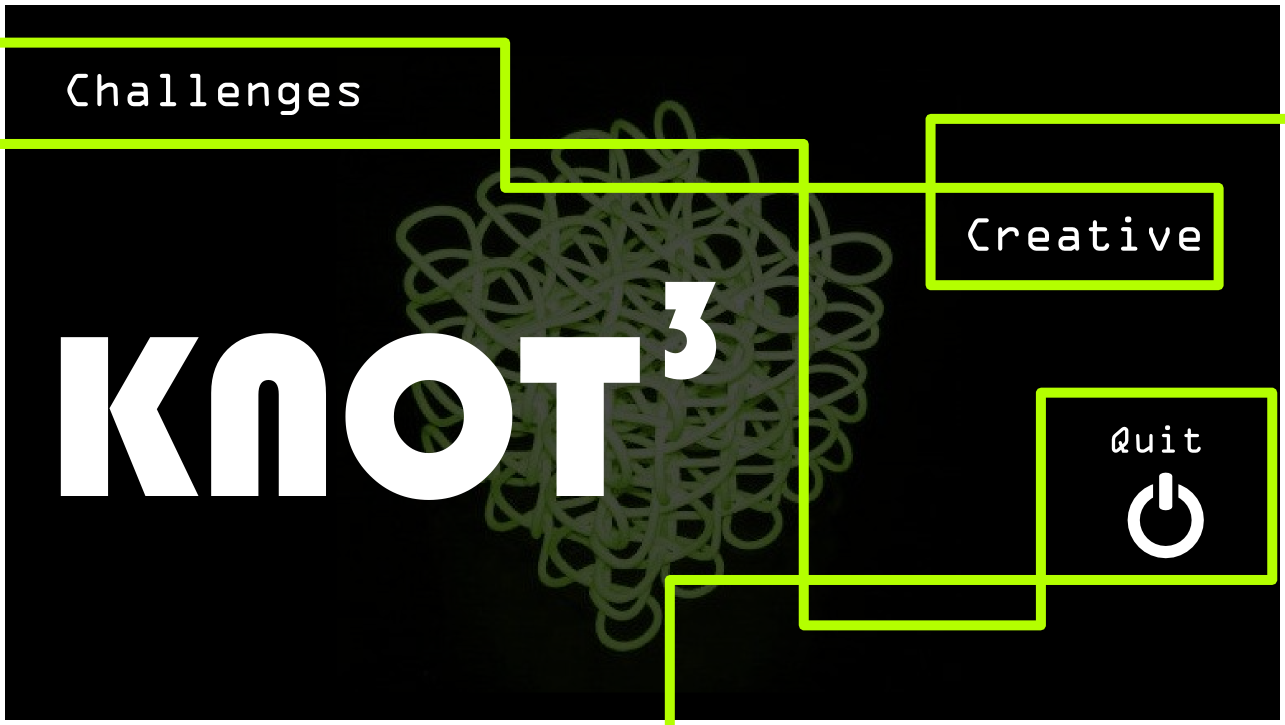
\includegraphics[width = 0.95\textwidth]{Inhalt/Nutzung/Grafiken/Grafische_Oberflaechen/01_Knot3-mainscreen.png}
	  \caption{Mögliches Hauptmenü /PGO\_0010/}
	\end{figure}

	\begin{figure}[ht]
	  \centering
	  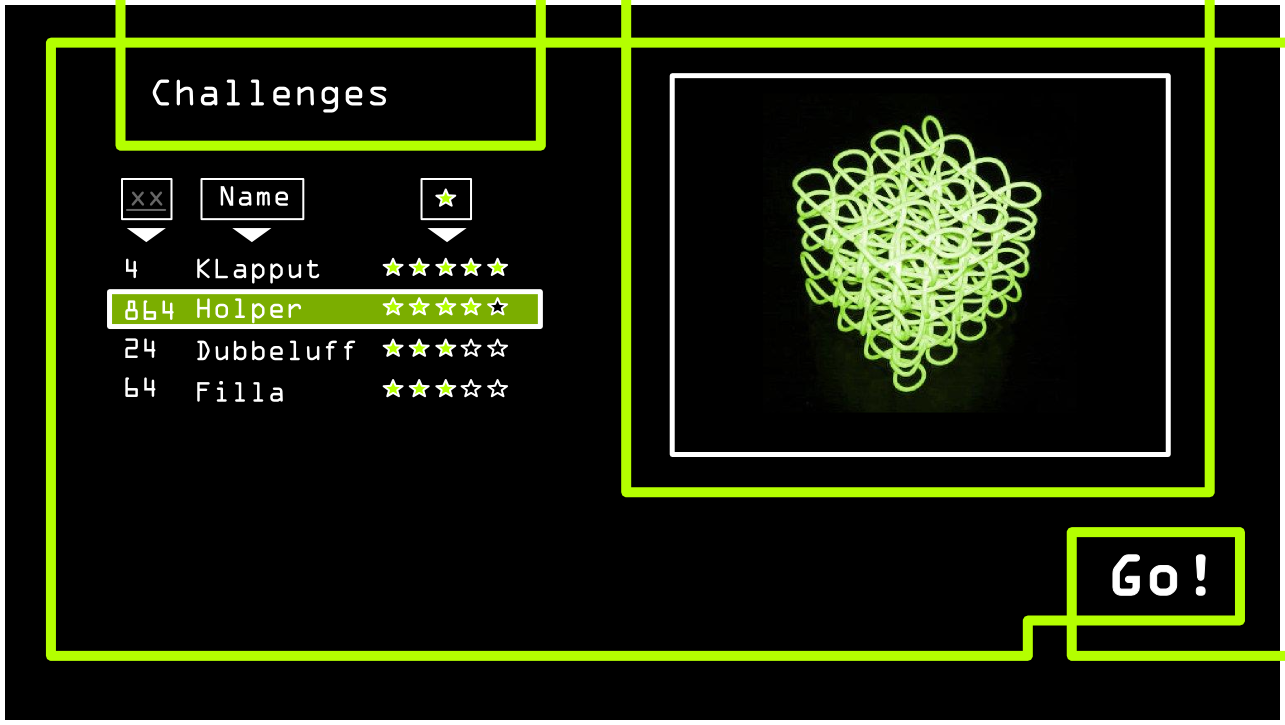
\includegraphics[width = 0.95\textwidth]{Inhalt/Nutzung/Grafiken/Grafische_Oberflaechen/04_Knot3-select-Challenge.png}
	  \caption{Auswahlmenü für die Herausforderungen /PGO\_0050/, mit Ausschnitt der Auswahlliste}
	\end{figure}
	
	\begin{figure}[ht]
	  \centering
	  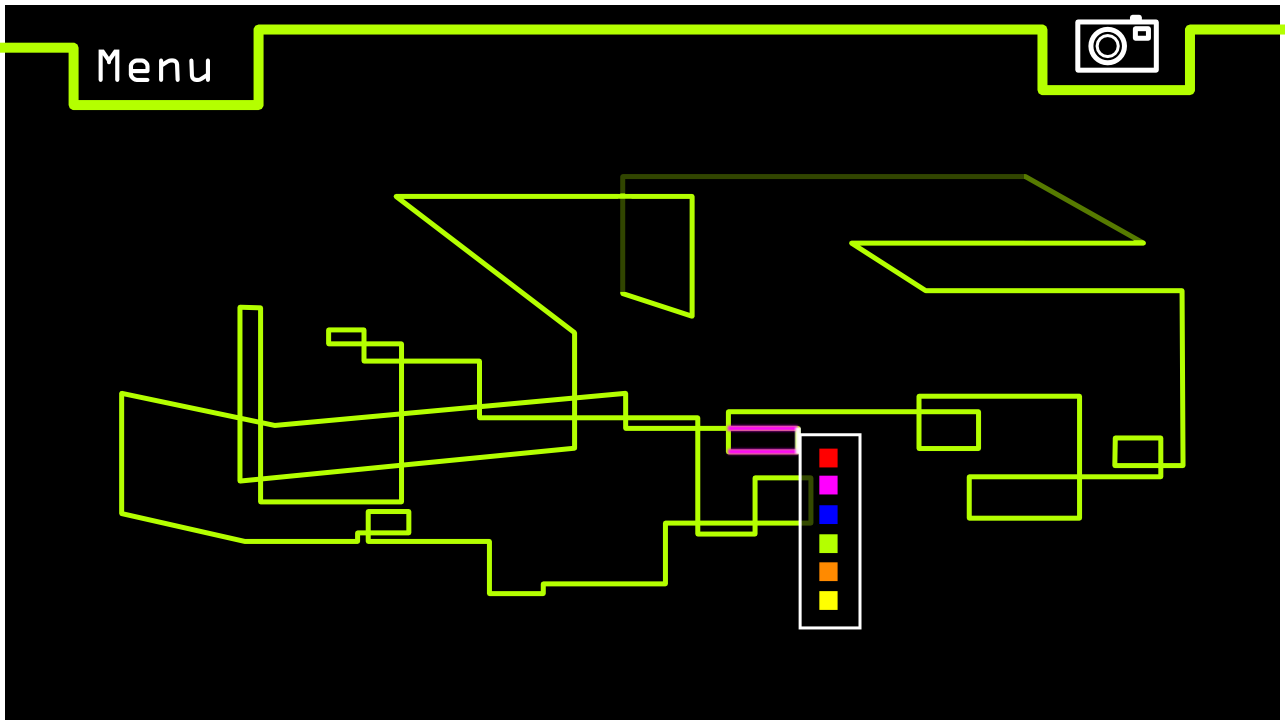
\includegraphics[width = 0.95\textwidth]{Inhalt/Nutzung/Grafiken/Grafische_Oberflaechen/05_Knot3-Colour-select.png}
	  \caption{Editoransicht /PGO\_1010/ mit geöffneter Farbauswahl zum Kanten einfärben /OFA\_200/.}
	\end{figure}
	
	\begin{figure}[ht]
	  \centering
	  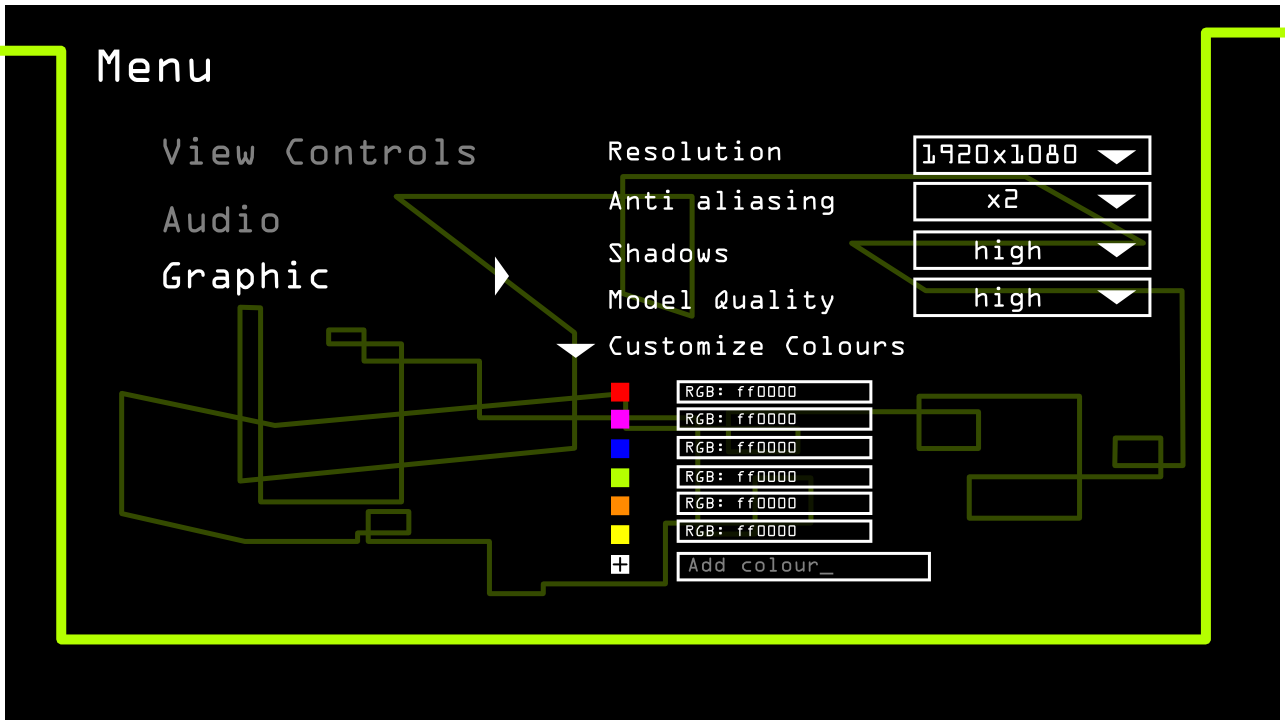
\includegraphics[width = 0.95\textwidth]{Inhalt/Nutzung/Grafiken/Grafische_Oberflaechen/08_Knot3-menu-graphics.png}
	  \caption{Mögliches Einstellungsmenü mit geöffnetem Untermenü für die Grafikeinstellungen. /OGO\_0020/ und /OGO\_0050/}
	\end{figure}


% !TeX encoding = UTF-8
%
% Interaktionsmodelle:
%


%
% Interaktionsmodelle starten auf eigener Seite.
%
\clearpage


\section{Interaktionsmodelle}
\label{NU:Interaktion}


\paragraph*{\underline{Pflicht:}}

\begin{ids}{\gls{PIM}}

	\id[10] In Menüs /PGO\_00XX/ und /PGO\_1030/ können Knöpfe und Auswahlflächen mit der Maus angeklickt werden.
	
	\id[20] Im Editor /PGO\_1010/ kann eine Kanten mit der Maus ausgewählt werden.
	
	\id[30] Durch drücken einer Taste kann /PIM\_20/ mehrfach ausgeführt werden, sodass die Auswahl aus mehreren Kanten besteht. Efüllt /PFA\_130/.
	
	\id[40] Durch gedrückt halten der Maustaste beginnen auf den Pfeilen in den Raumrichtungen /PFA\_355/ kann die durch /PIM\_20/ enstandene Auswahl in die entsprechende Raumrichtung verschoben werden. Erfüllt /PFA\_140/.
	
	\id[50] /PIM\_40 löst beim loslassen der Maustaste einen Transformationsschritt aus, für den es eine Visuelle Vorschau gibt /PFA\_310/.
	
	\id[60] Im Editor /PGO\_1010/ kann durch Tastendruck oder Mausklick auf eine Schaltfläche das Pausenmenü /PGO\_1030/ öffnen.
	
	\id[70] Im Editor /PGO\_1010/ ist Lineares verschieben des Kamerafokus in Blickrichtung und Senkrecht dazu ist über die Tastatur möglich.
	
	\id[80] Im Editor /PGO\_1010/ kann man den Kamerabstand zum Fokus (Zoom) über das Mausrad oder durch Tastendruck vergrößern und verkleinern.
	
	\id[90] Im Editor /PGO\_1010/ kann durch halten der rechten Maustaste die Kamera bei gleichbleibendem Fokus Kugelförmig darum bewegt werden.
	
	\id[100] Ist durch /PIM\_20/ eine Auswahl getroffen worden bleibt beim drehen /PIM\_90/ nicht der Fokus, sondern der Mittelpunkt der Auswahl an der gleichen Stelle.
	
	\id[110] Eine durch /PIM\_20/ getroffene Auswahl kann durch klick in den leren Raum aufgehoben werden.
	\id[120] Ein Tranformationsschritt /PIM\_50/ kann duch eine Tastenkombinatation oder einen Klick auch den "`undo"' Knopf rückgängig gemacht werden. Erfüllt /PFA\_160/.
	
	\id[130] Die Automatische Kameraführung /PK\_110/ dreht die Kamera und verschiebt den Fokus, sodass stets alle bisherigen Kanten und alle neu erstellten sichtbar sind und Platz für einfache transformationen bleibt.

\end{ids}


%
% Optionale Interaktionsmodelle starten auf einer eigenen Seite.
% nicht
%\clearpage


\paragraph*{\underline{Optional:}}

\begin{ids}{\gls{OIM}}

	\id[10] durch eine Tastenkombination oder einem Klick auf den "`redo"' Knopf kann eine rückgängig gemachte transformation /PIM\_120/ wieder hergestellt werden. Erfüllt /OFA\_190/.
	\id[20] Bei /PIM\_20/ ausgewählte Kanten kann durch Tastendruck ein auswahlmenü für personalisierte Farben aufgerufen werden.
	\id[30] Ein Klick auf eine Farbe im Farbauswahlmenü /OIM\_20/ färbt die ausgewählten Kanten in der Entsprechenden Farbe ein. Ein Klick in den leeren Raum schließt das Menü.
	\id[40] Im Editor /PGO\_1010/ ruft ein Klick auf den Knopf "`render/export"' oder ein passendes Icon das Menü für die Exportfunktionen /OGO\_1020/ auf.
	\id[50] Bei passender Auswahl durch /PIM\_20/ kann die eingeschlossene Fläche gefüllt werden. /OFA\_210/ 

\end{ids}


%\subsection*{\underline{Visualisierungen:}}

\begin{landscape}

	\begin{figure}[ht]
	% ssetpagelength
	  \centering
	  \includesvg[width = 1.2\textwidth]{inGame}
	  \caption{Interaktionen während eines Spiels (allgemein)}
	\end{figure}

\end{landscape}

\clearpage

%% !TeX encoding = UTF-8
%
% Interaktionsmodelle:
%


%
% Schnittstellen starten auf eigener Seite.
%
\clearpage


\section{Schnittstellen}
\label{NU:Schnittstellen}~\\

...
\\


\subsection*{\underline{Pflicht-Schnittstellen:}}

\begin{ids}{\gls{PSS}}

	\id[ 11] ... \hfill\\
	
	(Eine Schnittstelle) ...
	
	\id[100] ... \hfill\\
	
	(Eine Schnittstelle) ...

\end{ids}

~\\


%
% Optionale Schnittstellen starten auf einer eigenen Seite.
%
\clearpage


\subsection*{\underline{Optionale Schnittstellen:}}

\begin{ids}{\gls{OSS}}

	\id[ 11] ... \hfill\\
	
	(Eine Schnittstelle) ...
	
	\id[100] ... \hfill\\
	
	(Eine Schnittstelle) ...

\end{ids}




%
%	Grafiken einbinden: ("Hier.")
%
%	\begin{figure}[ht]
%		\includegraphics[width=\textwidth]{.}
%	\end{figure}
%	

%
%	Grafiken einbinden: ("Hier!")
%
%	\begin{figure}[!ht]
%		\includegraphics[width=\textwidth]{.}
%	\end{figure}
%

	% !TeX encoding = UTF-8
%
% Produkt-Qualitätssicherung
%


\chapter{Qualitätssicherung}
\label{Qualitätssicherung}


\section{Prioritäten}

...
\\


\section{Testfälle}

\subsection{Pflicht-Testfälle}

...
\\


\subsection{Optionale Testfälle}

...
\\

	% !TeX encoding = UTF-8
%
% Produkt-Entwicklung
%


\chapter{Entwicklung}
\label{EW}~\\


\section{Umgebung}
\label{EW:Umgebung}

...
\\


\subsection{Hardware}


\subsubsection*{Mindestanforderungen}

...
\\


\subsection{Software}

\subsubsection*{Mindestanforderungen}

...
\\



%\section{Organisation}
%\label{EW:Organisation}
%
%...
%\\


 % !!!
	% !TeX encoding = UTF-8
%
% Produkt-Verteilung
%


\chapter{Verteilung}
\label{VT}~\\

(Wie das Produkt verteilt wird) ...


	
	% Verzeichnisse
	%
	% !TeX encoding = UTF-8
%
% Verzeichnisse
%


\chapter{Verzeichnisse}
\label{Verzeichnisse}


\gls{gfa:wbrot}

\setglossarysection{section}
\printglossary[numberedsection, title = Fachausdrücke]



\printglossary[numberedsection, title = Abkürzungen]



	
	% Anhänge
	%
	%
% Anh�nge
%


\chapter{Anh�nge}
\label{Anh�nge}













	
	% Schluss-Teaser
	%
	% !TeX encoding = UTF-8


\end{document}